\documentclass[12pt]{article}
\usepackage[margin=1in]{geometry}
\usepackage[all]{xy}
\usepackage{hyperref}
\hypersetup{
    colorlinks=true,
    linkcolor=blue,
    filecolor=magenta,      
    urlcolor=cyan,
    pdftitle={Overleaf Example},
    pdfpagemode=FullScreen,
    }


\usepackage{amsmath,amsthm,amssymb,color,latexsym}
\usepackage{geometry}        
\geometry{letterpaper}    
\usepackage{graphicx}

\newtheorem{problem}{Problem}

\newenvironment{solution}[1][\it{Solution}]{\textbf{#1. } }{$\square$}


\begin{document}
\noindent VE3310-1 23H Operativsystemer VG \hfill Coordinate frames \#\\
Edvart Bjerke. (23.10.2023)

\hrulefill

\subsection*{Coordinate frames}
\subsubsection*{Problem Statement}

The goal of this assignment was to implement ROS (Robot Operating System) nodes 
for tracking the position and orientation of a flying drone in 3D space. More specifically, use the tf 
library to broadcast the transformation from some fixed point of reference to the drone's position and orientation.
To accomplish this, a combination of UWB (Ultra Wide Band) beacons, UWB tags and the drone's embedded IMU module was used.

\subsubsection*{Hardware and configuration}
\begin{enumerate}
    \item Decawave UWB beacons
    \item Decawave UWB tags
    \item Tello Drone
    \item Drone Battery
    \item Laptop
    \item Android device
\end{enumerate}

The Decawave beacons were set up in the corners of a small room, and by measuring the relative positions of four UWB beacons, a localization network was established. To track the drone, a UWB tag is attached to the physical drone, powered by its internal battery.
The UWB system provides positional tracking of the drone (up to 10Hz), while the drone's embedded INS system provides intertial data such as a quaternion orientation, angular velocities and linear accelerations, at a high update rate.
A final UWB device is connected to the laptop, serving as an interface for processing the tag positions programatically.

\subsubsection*{Software}
The software is implemented in Python using the ROS framework, particularly leveraging the tf library. Pre-existing code is responsible for the publishing of the drone's inertial data and the UWB tag positional data.
Since the beacons are assumed to be stationary, the \textit{static\_transform\_publisher} node of the tf library is used to establish the transforms from the fixed origin to the four stationary UWB beacons. 
\\

The origin was chosen to be below one of the beacons, at ground level.
Since the drone is not stationary, a dynamic transform node has been implemented. It consists of two subscribers, one for the positional data and one for the orientation. The positional data is given in standard $(x, y, z)$ euclidean coordinates, while the orientation has a quaternion $(q_0, q_1, q_2, q_3)$ representation.
Because of quaternion convention differences between ROS and Tello, the broadcasted quaternion vector is modified to be $(q_3, q_0, -q_1, -q_2)$. 
\\

The transform from the origin to the drone is then broadcasted on every new position or orientation update.
Since the Tello drone yaw reference is initialized to 0 at startup, there is no deterministic way to know a world-referenced yaw angle, unless the drone is initialized at a known angle (for example, towards north). 
This could be important if we want to send room-relative or geographic coordinates to the drone, but is not important if the waypoints are relative to the pose of the drone.
The code can be found on the github repo: \url{https://github.com/Autonomi-USN/Tello/tree/edvart/tello_tf}

\subsubsection*{Results}
\begin{figure}[h]
    \centering
    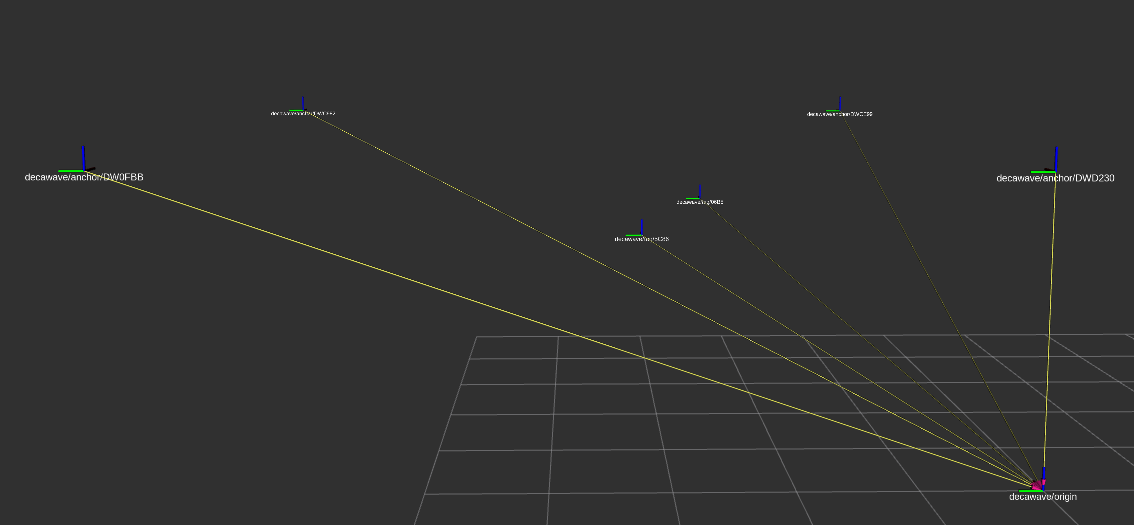
\includegraphics[width=0.8\textwidth]{figures/image1.png}
    \label{fig:frames1}
\end{figure}
\begin{figure}[h]
    \centering
    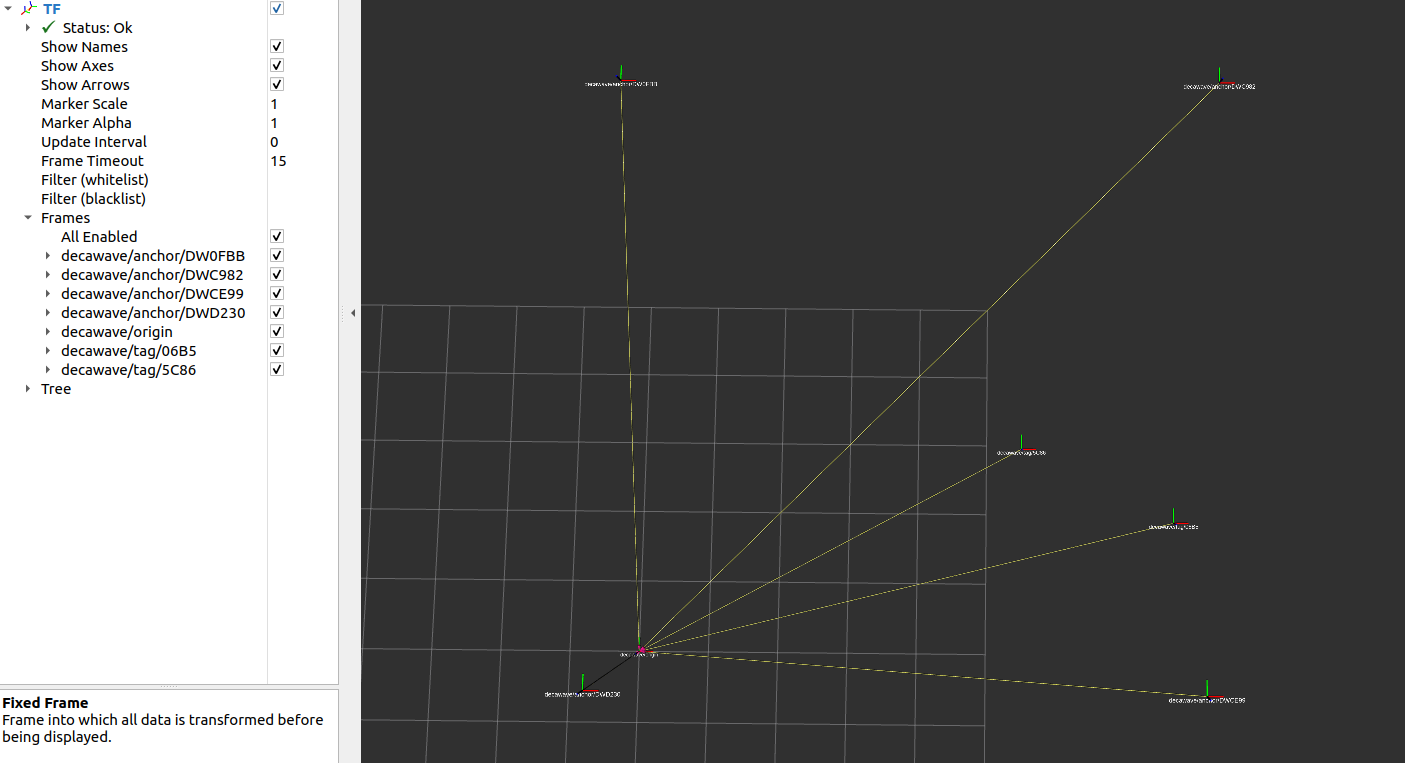
\includegraphics[width=0.8\textwidth]{figures/image.png}
    \caption{Visualization of the localization network in RViz. The network consists of the ground-level origin, four UWB beacons (corners) and two UWB tags.}
    \label{fig:frames2}
\end{figure}
\begin{figure}[h]
    \centering
    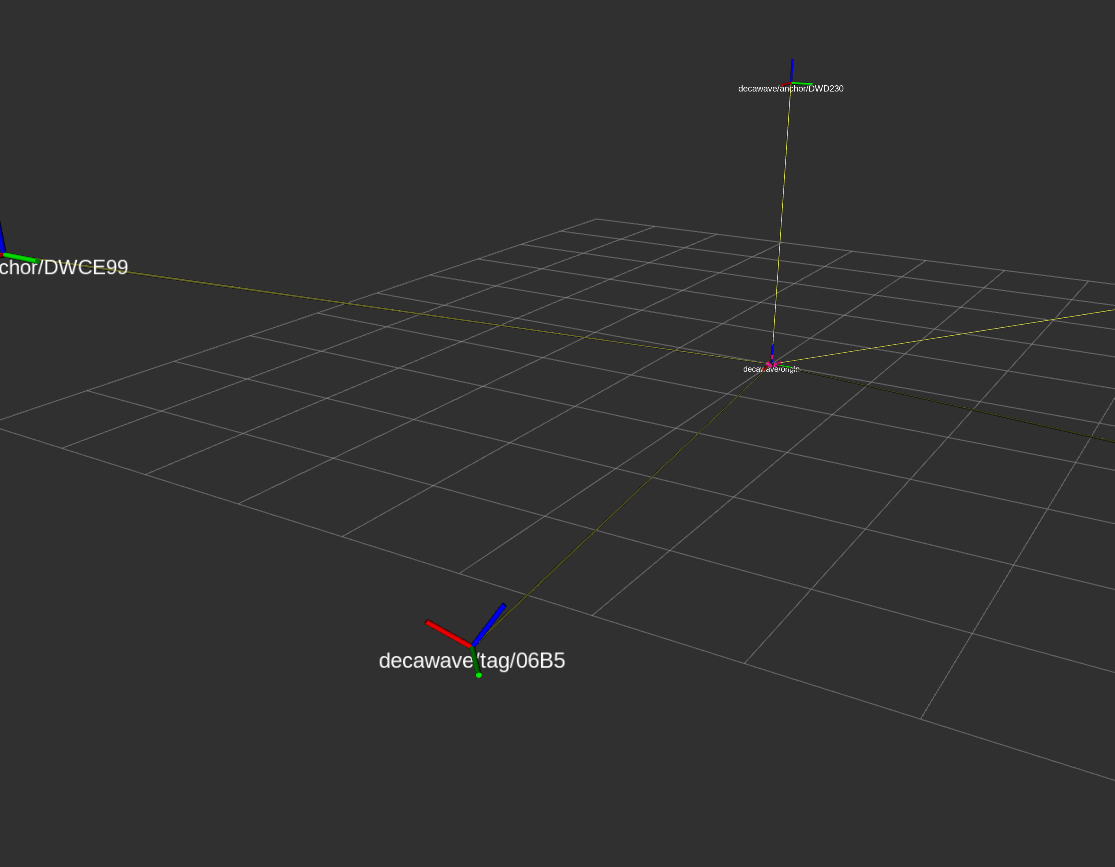
\includegraphics[width=0.8\textwidth]{figures/image2.png}
    \caption{Position and orientation of a drone in RViz.}
    \label{fig:frames3}
\end{figure}

\end{document}